\documentclass[11pt]{article}

\def\shownotes{1}
\def\notesinmargins{0}

\usepackage{fullpage}

\usepackage{mathtools,color,xcolor,hyperref,graphicx,wrapfig,listings,array,xspace}
\usepackage{caption}
\usepackage{subcaption}

\usepackage{amsfonts}
% https://tex.stackexchange.com/questions/11719/how-do-i-backcolor-in-verbatim
\usepackage{xcolor}
\usepackage{alltt}
% Compensate for fbox sep:
\newcommand\Hi[2][lightgray]{%
	\hspace*{-\fboxsep}%
	\colorbox{#1}{#2}%
	\hspace*{-\fboxsep}%
}

\ifnum\shownotes=1
\ifnum\notesinmargins=1
\newcommand{\authnote}[2]{\marginpar{\parbox{\marginparwidth}{\tiny %
  \textsf{#1 {\textcolor{blue}{notes: #2}}}}}%
  \textcolor{blue}{\textbf{\dag}}}
\else
\newcommand{\authnote}[2]{
  \textsf{#1 \textcolor{blue}{: #2}}}
\fi
\else
\newcommand{\authnote}[2]{}
\fi

\newcommand{\lnote}[1]{{\authnote{\textcolor{orange}{Leo notes}}{#1}}}
\newcommand{\snote}[1]{{\authnote{\textcolor{yellow}{Scalahub notes}}{#1}}}
\newcommand{\knote}[1]{{\authnote{\textcolor{green}{kushti notes}}{#1}}}
\newcommand{\mnote}[1]{{\authnote{\textcolor{red}{Morphic}}{#1}}}
\newcommand{\dnote}[1]{{\authnote{\textcolor{brown}{Dima notes}}{#1}}}

\newcommand{\ret}{\mathsf{ret}}
\newcommand{\new}{\mathsf{new}}
\newcommand{\hnew}{h_\mathsf{new}}
\newcommand{\old}{\mathsf{old}}
\newcommand{\op}{\mathsf{op}}
\newcommand{\verifier}{\mathcal{V}}
\newcommand{\prover}{\mathcal{P}}
\newcommand{\key}{\mathsf{key}}
\newcommand{\nextkey}{\mathsf{nextKey}}
\newcommand{\node}{\mathsf{t}}
\newcommand{\parent}{\mathsf{p}}
\newcommand{\leaf}{\mathsf{f}}
\newcommand{\vl}{\mathsf{value}}
\newcommand{\balance}{\mathsf{balance}}
\newcommand{\lft}{\mathsf{left}}
\newcommand{\rgt}{\mathsf{right}}
\newcommand{\lbl}{\mathsf{label}}
\newcommand{\direction}{\mathsf{d}}
\newcommand{\oppositedirection}{\bar{\mathsf{d}}}
\newcommand{\found}{\mathsf{found}}
\newcommand{\mypar}[1]{\smallskip\noindent\textbf{#1.}\ \ \ }
\newcommand{\ignore}[1]{}

\newcommand{\langname}{ErgoScript\xspace}
%\newcommand{\mixname}{ZeroJoin\xspace}
\newcommand{\mixname}{ErgoMix\xspace}
%\newcommand{\mixname}{ErgoJoin\xspace}


\newcommand{\lst}[1]{\text{\lstinline[basicstyle={\ttfamily}]$#1$}}

\newcommand{\andnode}{\ensuremath{\mathsf{AND}}}
\newcommand{\ornode}{\ensuremath{\mathsf{OR}}}
\newcommand{\tnode}{\ensuremath{\mathsf{THRESHOLD}}}
\newcommand{\GF}{\ensuremath{\mathrm{GF}}}


\begin{document}

\title{Advanced \langname Tutorial}

%\title{Protocols in \langname: From Games to Mixers}

\author{Ergo Developers}


\maketitle


\begin{abstract}
%This article describes \langname via examples. 
Ergo is a smart contract platform based on Bitcoin's UTXO model and Ethereum-like functionality that it provides via a language called \langname. The syntax of \langname is a subset of Scala's. In this article, we give a high-level overview of \langname using examples.

% Note that certain contracts of \langname  (such as \mixname in Section~\ref{mix}) cannot be easily ported to Ethereum due to its account-based model (as opposed to UTXOs)


We use \langname to create smart contracts for several protocols such as an XOR game, a rock-paper-scissors game, {\em reversible addresses} that have anti-theft features, and {\em \mixname}, a privacy enhancing protocol, which can be considered a non-interactive variant of CoinJoin. % and an improved variant of ZeroCoin. 

%We create several protocols using \langname, such as games and mixing protocols. 
\end{abstract}

\section{Introduction}

\ignore{
\subsection{$\Sigma$-Protocols}
\label{intro:sigma}

The classic example of a $\Sigma$-protocol is the Schnorr identification scheme~\cite{Sch91}. Let $G$ be a cyclic multiplicative group of prime order $q$ and $g$ a generator of $G$. Assume that computing discrete logarithms in $G$ is hard. Alice has a secret $x \in \mathbb{Z}_q$, which she wants to prove knowledge of to some Bob who knows $u = g^x$.

\begin{enumerate}
	\item \textbf{Commit:} Alice selects a random $r$, computes $t = g^r$ and sends $t$ to Bob.
	\item \textbf{Challenge:} Bob selects a random $c\in\mathbb{Z}_q$ and sends $c$ to Alice.
	\item \textbf{Response:} Alice computes $z = r + cx$ and sends $z$ to Bob. Bob accepts iff $g^z = t\cdot u^c$.
\end{enumerate}

The above protocol is a proof of knowledge because Bob can extract $x$ if he can get Alice to respond twice for the same $r$ and different $c$. As an example, for $c = 1, 2$, Bob can obtain $r+x$ and $r+2x$, the difference of which gives $x$. This is also called (special) soundness. The above protocol is also (honest verifier) zero-knowledge because anyone can impersonate Alice if the challenge $c$ of Step 2 is known in advance, simply by picking random $z \in\mathbb{Z}_q$ and computing $t = g^z/u^c$. The statement ``I know the discrete log of $u$ to base $g$'' is called the {\em proposition}, which we denote by $\tau$.

Any protocol that has the above 3-move structure (Alice $\stackrel{t}{\rightarrow}$ Bob, Bob $\stackrel{c}{\rightarrow}$ Alice, Alice $\stackrel{z}{\rightarrow}$ Bob), along with zero-knowledge and soundness property is called a $\Sigma$-protocol. 

\subsection{$\Sigma$-Proofs}
For any $\Sigma$-protocol with messages $(t, c, z)$, we can apply the Fiat-Shamir transform~\cite{fiatshamir} to convert it into a non-interactive one by replacing the role of Bob in Step 2 by any hash function $H$ and computing $c$ = $H(t)$. The resulting protocol with messages $(t, H(t), z)$ can be performed by Alice alone. Intuitively, since $c$ depends deterministically on $t$, Bob cannot ``rewind'' Alice and get two different responses for the same $r$. Additionally, Alice cannot know $c$ in advance before deciding $t$ if $H$ behaves like a random oracle. We call such a non-interactive proof a {\em $\Sigma$-proof}~\cite{Cra96} .

Conceptually, $\Sigma$-proofs are generalizations of digital signatures~\cite{CL06}.
In fact, Schnorr signature scheme~\cite{Sch91} (whose more recent version is popularly known as EdDSA \cite{BDLSY12,rfc8032}) is a special case of the above identification protocol with $c = H(t \Vert m)$, where $m$ is the message. The signature proves that the recipient knows the discrete logarithm of the public key (the proof is attached to a specific message, such as a particular transaction, and thus becomes a signature on the message; all $\Sigma$-proofs described here are attached to specific messages). $\Sigma$-proofs exist for proving a variety of properties and, importantly for \langname, elementary $\Sigma$-proofs can be combined into more sophisticated ones using the techniques of \cite{CDS94}. 
}

%\section{Overview of \langname}
 
\ignore{
Although \langname uses $\Sigma$-protocols, it does so transparently and developers are not required to understand them. 
Here we briefly describe \langname ``under the hood'' -- how it works and what primitives it uses.


\subsection{Complex $\Sigma$-Protocols}

Any two $\Sigma$-protocols of propositions $\tau_0, \tau_1$ with messages $(t_0, c_0, z_0), (t_1, c_1, z_1)$ respectively can be combined into a $\Sigma$-protocol of $\tau_0 \land \tau_1$ with messages $(t, c, z) = (t_0\Vert t_1,c_0\Vert c_1, c_0\Vert c_1)$. We call such a construction an $\andnode$ operator on the protocols. 
More interestingly, as shown in \cite{CDS94},the two protocols can also be used to construct a $\Sigma$-protocol for $\tau_0\lor \tau_1$, where Alice proves knowledge of the witness of one proposition, without revealing which. Let $b\in \{0, 1\}$ be the bit such that Alice knows the witness for $\tau_b$ but not for $\tau_{1-b}$. Alice will run the correct protocol for $\tau_b$ and a simulation for $\tau_{1-b}$. First she generates a random challenge $c_{1-b}$. She then generates $(t_{1-b}, z_{1-b})$ by using the simulator on $c_{1-b}$. She also generates $t_b$ by following the protocol correctly. The pair $(t_0, t_1)$ is sent to Bob, who responds with a challenge $c$. Alice then computes $c_b = c\oplus c_{1-b}$. She computes $z_b$ using $(t_b, c_b)$. Her response to Bob is $((z_0, c_0), (z_1, c_1))$, who accepts if: (1) $c = c_0 \oplus c_1$ and (2) $(t_0, c_0, z_0), (t_1, c_1, z_1)$ are both accepting convesations for $\tau_0, \tau_1$ respectively. We call such a construction an $\ornode$ operator. 

Clearly, both the $\andnode$ and $\ornode$ operators also result in $\Sigma$-protocols that can be further combined or made non-interactive via the Fiat-Shamir transform. 

There is one more operator that we need called $\tnode$, which allows us to construct a $k$-out-of-$n$ $\Sigma$-protocol~\cite{CDS94} as follows. Given $n$ propositions, Alice can prove knowledge of witnesses for at least $k$ propositions without revealing which. 

\langname gives the ability to build more sophisticated $\Sigma$-protocols using the connectives $\andnode$, $\ornode$, and $\tnode$. 
Crucially, the proof for an $\ornode$ and a $\tnode$ connective does not reveal which of the relevant values the prover knows. For example, in \langname a ring signature by public keys $u_1, \dots, u_n$ can be specified as an $\ornode$ of $\Sigma$-protocols for proving knowledge of discrete logarithms of $u_1, \dots, u_n$. The proof can be constructed with the knowledge of just one such discrete logarithm, and does not reveal which one was used in its construction. 

\subsection{Other Features of \langname} 
}

A key feature of \langname is the use of {\em Sigma-Protocols} (written $\Sigma$-protocols)\cite{Dam10} interleaved with predicates on the transaction and the blockchain state. \langname currently supports two such-Protocols defined on a group $G$ of prime order $q$, written here in multiplicative form. 
%This group is exactly the one defined by the secp256k1 curve of Bitcoin. 
The first, denoted as \texttt{proveDlog(u)}, is a {\em proof of knowledge of Discrete Logarithm} of some arbitrary group element $u$ with respect to a fixed generator $g$, where the spender proves knowledge of $x$ such that $u = g^x$.
This is derived from Schnorr signatures~\cite{Sch91}. The second, denoted as \texttt{proveDHTuple}, is a {\em proof of knowledge of Diffie-Hellman Tuple} and is explained in Section~\ref{mix}.


The main structure in \langname is a \emph{box}, which is roughly like a UTXO of Bitcoin. A transaction spends (destroys) some boxes by using them as inputs and creates new boxes as outputs.  \langname is used to write the {\em spending condition} protecting funds stored in a box. The spender of a box must provide a `proof' of satisfying that condition. 

%A box is made of upto ten {\em registers} labelled $R_0, R_1,\ldots R_9$, four of which are mandatory. $R_0$ contains the monetary value, $R_1$ contains a script with the spending condition, $R_2$ contains assets (tokens) and $R_3$ contains a unique identifier of 34 bytes made up of a transaction ID (32 bytes) and an output index (2 bytes). The other registers can contain any data or be empty (ensuring that no empty register has index lower than a non-empty one).

% Under the hood, \langname is compiled to {\em ErgoTree}, which is what an Ergo node understands. 

%In addition to $\Sigma$-protocols, \langname allows for predicates over the state of the blockchain and the current transaction. These predicates can be combined, via Boolean connectives, with $\Sigma$-statements, and are used during transaction validation. 
%The set of predicates is richer than in Bitcoin, but still lean in order to allow for efficient processing even by light clients. Like in Bitcoin, we allow the use of current height of the blockchain; unlike Bitcoin, we also allow the use of information contained in the spending transaction, such as inputs it is trying to spend and outputs it is trying to create. This feature enables self-replication and sophisticated (even Turing-complete) long-term script behaviour, as described in examples below.


The following sections present smart contracts using \langname. More details of \langname are available in the white paper~\cite{whitepaper} and the code for the below examples is available on GitHub~\cite{langrepo}. 
\section{Basic Examples: Enhanced Spending Contracts}

The examples below use P2SH address and highlight some limitation of Bitcoin. 

\subsection{Short-lived Unconfirmed Transactions: Paying for Coffee}

Alice is paying for coffee using cryptocurrency. She makes a payment but it is taking a long time for the transaction to confirm. She decides to pay using cash and leave. However, she is worried that her original payment will eventually confirm and then she will either lose it or have to ask for a refund. In Bitcoin, she can try to double spend the transaction, which is not always guaranteed, even if using {\em replace-by-fee}. \langname has a better solution using {\em timed-payments} so that if the transaction is not confirmed before a certain height, it is no longer valid. Timed-payments require Alice's funds be stored in a {\em timed address}, which is the P2SH of the following script: 

%Assume \texttt{bob} is the coffee shop public key and Alice is the customer paying for coffee.
\begin{verbatim}
alice && HEIGHT <= getVar[Int](1).get
\end{verbatim}

Here \texttt{alice} is a {\em named constant} representing her public key.
Any funds deposited to this address can only be spent if the spending transaction satisfies following:
\begin{enumerate}
	\item Context variable with id 1 of the box being spent must contain an integer, say $i$.
	\item The height at mining should be less than or equal to $i$. 
\end{enumerate}

Observe that if the transaction is not mined before height $i$ then the transaction becomes invalid. When paying at a coffee shop, for example, Alice can set $i$ close to the height $h$ at the time of broadcast, for instance, $i = h + 10$. 
Alice can still send non-timed payments by making $i$ very large. Since the context variables are part of the message in constructing the zero-knowledge proof, a miner cannot change it (to make this transaction valid). 

\subsection{Hot-Wallet Contracts: Reversible Addresses}

We create a useful primitives called {\em reversible addresses}, designed for storing funds in a hot-wallet. %These addresses have anti-theft features in the following sense:
Any funds sent to a reversible address can only be spent in way that allows payments to be reversed for a certain time. The idea was proposed for Bitcoin~\cite{raddress} (using the moniker {\em R-addresses}) and requires a hardfork. In \langname, however, this can be done natively.

To motivate this feature, consider managing the hot-wallet of a mining pool or an exchange. Funds withdrawn by customers originate from this hot-wallet. Being a hot-wallet, its private key is succeptible to compromise. One day you discover several unauthorized transactions from the hot-wallet, indicating a breach. You wish there was a way to reverse the transactions and cancel the withdraws but alas this is not the case. In general there is no way to recover the lost funds once the transaction is mined, even if the breach was discovered within minutes. 
%The irreversibility of fund transfers, usually considered a feature, has now become a bug.

We would like that in the event of such a compromise, we are able to save all funds stored in this wallet and move them to another address, provided that the breach is discovered within a specified time (such as 24 hours) of the first unauthorized withdraw. 

To achieve this, we require that all coins sent from the hot-wallet (both legitimate and by the attacker)
have a 24 hour cooling-off period, during which the created boxes can only be spent by a trusted private key that is was selected {\em before} the compromise occurred. This trusted key must be different from the hot-wallet private key and should ideally be in cold storage. 
After 24 hours, these boxes become `normal' and can only be spent by the receiver.

This is done by storing the hot-wallet funds in a special type of address denoted as {\em reversible}. Assume that \texttt{alice} is the public key of the hot-wallet and \texttt{carol} is the public key of the trusted party. Note that the trusted party must be decided at the time of address generation and cannot be changed later. To use a different trusted party, a new address has to be generated. Let \texttt{blocksIn24h} be the estimated number of blocks in a 24 hour period. A reversible address is a P2SH
%\footnote{As in Bitcoin, a P2SH (Pay to Script Hash) address is created from the hash of a script encoding spending conditions for any UTXOs controlled by that address.} 
address whose script encodes the following conditions:   
\begin{enumerate}
	\item This input box can only be spent by \texttt{alice}.
	\item Any output box created by spending this input box must have in its register $R_5$ a number at least \texttt{blocksIn24h} more than the current height. 
	\item Any output box created by spending this input box must be protected by a script requring the following: 	
	\begin{enumerate}
		\item Its register $R_4$ must have an arbitrary public key called \texttt{bob}.
		\item Its register $R_5$ must have an arbitrary integer called \texttt{bobDeadline}.
		\item It can only be spent spent by \texttt{carol} if \texttt{HEIGHT $\leq$ bobDeadline}.
		\item It can only be spent by \texttt{bob} if \texttt{HEIGHT $>$ bobDeadline}.
	\end{enumerate}  
\end{enumerate}

Thus, all funds sent from such addresses have a temporary lock of \texttt{blocksIn24h} blocks. This can be replaced by any other desired value but it must be decided at the time of address generation. 
Let \texttt{bob} be the public key of a customer who is withdrawing. The sender (\texttt{alice}) must ensure that register $R_4$ of the created box contains \texttt{bob}. In the normal scenario, \texttt{bob} will be able to spend the box after roughly \texttt{blocksIn24h} blocks (with the exact number depending on \texttt{bobDeadline}). 

If an unauthorized transaction from \texttt{alice} is detected, an ``abort procedure'' is triggered via \texttt{carol}: all funds sent from \texttt{alice} and in the locked state are suspect and need to diverted elsewhere. %Additionally, boxes currently controlled by \texttt{alice} also need to be sent secure addresses. 

%Such addresses are designed for storing large amount of funds for automated withdraws (such as hot-wallets). 
%They are not designed for daily spending (such as paying for a coffee). 
To create a reversible address, first create a script, \texttt{withdrawScript}, with the following code:
\begin{verbatim}
val bob         = SELF.R4[SigmaProp].get // public key of customer withdrawing
val bobDeadline = SELF.R5[Int].get       // max locking height
(bob && HEIGHT > bobDeadline) || (carol && HEIGHT <= bobDeadline)
\end{verbatim}

Let \texttt{feeProposition} be the script of a box that pays mining fee and \texttt{maxFee} be the maximum fee allowed in one transaction. The reversible address is the P2SH address of the following script:
\begin{verbatim}
val isChange = {(out:Box) => out.propositionBytes == SELF.propositionBytes}
val isWithdraw = {(out:Box) => 
  out.R5[Int].get >= HEIGHT + blocksIn24h && 
  out.propositionBytes == withdrawScript
}
val isFee = {(out:Box) => out.propositionBytes == feeProposition}
val isValid = {(out:Box) => isChange(out) || isWithdraw(out) || isFee(out)}

val totalFee = OUTPUTS.fold(0L, {
    (x:Long, b:Box) => if (isFee(b)) x + b.value else x 
  }
)
alice && OUTPUTS.forall(isValid) && totalFee <= maxFee
\end{verbatim}

\subsection{Cold-Wallet Contracts: Limiting Spending Capacity}

Assume an address is protected by 2 private keys, corresponding to the public keys \texttt{alice} and \texttt{bob}. For security, we want the following conditions to hold:

\begin{enumerate}
	\item One key can spend at most 1\% or 100 Ergs (whichever is higher) in one day.
	\item If both keys are spending then there are no restrictions. 
\end{enumerate}

Let \texttt{blocksIn24h} be the number of blocks in 24 hours. Instead of hardwiring 1\% and 100 Ergs, we will use the named constants \texttt{percent} and \texttt{minSpend} respectively. The cold-wallet address is the P2SH address of the following script:
\begin{verbatim}
val storedStartHeight = SELF.R4[Int].get // block at which the period started
val creationHeight = SELF.creationInfo._1 // creation height
val startHeight = min(creationHeight, storedStartHeight) 
val notExpired = HEIGHT - startHeight <= blocksIn24h // expired if 24 hrs passed
val min = SELF.R5[Long].get // min Balance needed in this period

val ours:Long = SELF.value - SELF.value * percent / 100
val keep = if (ours > minSpend) ours else 0L // topup should keep min >= keep
val nStart:Int = if (notExpired) start else HEIGHT
val nMin:Long = if (notExpired) min else keep

val out = OUTPUTS(0)  
val valid = INPUTS.size == 1 && out.propositionBytes == SELF.propositionBytes &&
  out.value >= nMin && out.R4[Int].get >= nStart && out.R5[Long].get == nMin})
    
(alice && bob) || ((alice || bob) && min >= keep && (nMin == 0 || valid))
\end{verbatim}

Spending from this address is done in periods of 24 hours or more such that the maximum spendable is a fixed fraction of the amount at the beginning of the period. We do this by requiring the spending transaction to have an output with value greater than the minumum (which is stored in $R_5$) and paying back to the same address. The start of the current period is stored in $R_4$. Both registers are copied to the new output within the same period and get new values for if the current period has expired.


%\subsection{Advanced Cold-Wallet Contracts}
%
%We can extend the 2-party cold-wallet contract by adding a third party and the following conditions:
%
%\begin{enumerate}
%	\item One key can spend at most 1\% or 100 Ergs (whichever is higher) in one day.
%	\item For two keys the amount is 10\% or 1000 Ergs (whichever is higher).
%	\item If all three two keys are spending then there are no restrictions. 
%\end{enumerate}
\ignore{
\subsection{Revenue Sharing Contracts}

Assume that Alice, Bob and Carol agree to share revenue with a 50\%, 30\% and 20\% ratio respectively. The following describes a contract that automatically enforces this for any coins sent to it. Let \texttt{outputScriptHash} be the hash of the following script:
		
%First create a script and compute its hash:
% There may be advantages of storing the public keys in a register rather than hardwiring them to address
%First add the public keys \texttt{alice}, \texttt{bob}  and \texttt{carol} of type \texttt{proveDlog} into the environment \texttt{env}. First create a script. 

%First create an outputScript = 

\begin{verbatim}
val spenders = SELF.R4[Coll[(SigmaProp, Int)]].get
val index = getVar[Int](1).get // index of current spender 
val pubKey:SigmaProp = spenders(index)._1 // pub key of current spender
val ratio:Int = spenders(index)._2 // ratio of current spender
val total = spenders.fold(0, {(accum:Int, s:(SigmaProp, Int)) => accum + s._2})
val balance = SELF.value - SELF.value / total * ratio
val remainingSpenders = spenders.filter({(s:(SigmaProp, Int)) => s._1 != pubKey})
val outSpenders = OUTPUTS(0).R4[Coll[(SigmaProp, Int)]].get
val validOut = OUTPUTS(0).propositionBytes == SELF.propositionBytes &&
               OUTPUTS(0).value >= balance && remainingSpenders == outSpenders
pubKey && (outSpenders.size == 0 || validOut)
\end{verbatim}

The revenue sharing contract is encoded in the P2SH address of the following script: 
\begin{verbatim}
val spenders = Coll((alice, 50), (bob, 30), (carol, 20))
val index = getVar[Int](1).get // index of current spender 
val pubKey:SigmaProp = spenders(index)._1 // pub key of current spender
val ratio:Int = spenders(index)._2 // ratio of current spender
val balance = SELF.value - SELF.value / 100 * ratio  // Assume total is 100
val remainingSpenders = spenders.filter({(s:(SigmaProp, Int)) => s._1 != pubKey})
val outSpenders = OUTPUTS(0).R4[Coll[(SigmaProp, Int)]].get
val validOut = OUTPUTS(0).propositionBytes == outputScriptHash &&
               OUTPUTS(0).value >= balance && remainingSpenders == outSpenders
pubKey && validOut
\end{verbatim}

For any funds sent to this address, each party can spend only its share and must create another box with the balance amount that enforces the same condition for the remaining spenders.

%\subsection{Automated Salary Contracts}
%further improvements. Can we reduce offchain data size, do multiple mixes offchain?
}

\section{Two-party Protocols}

We focus on two-round, two-party protocols. %That is, protocols with two parties that can be performed in two transactions. 
In the first round, the first party, Alice, initiates the protocol by creating a box  protected by a script encoding the protocol rules. In the second round, the second party, Bob, completes the protocol by spending Alice's box usually with one of his own and creating additional boxes that encode the final state of the protocol. 

All the protocols here allow the first round to be offchain in the sense that Alice's box creation may be deferred until the time Bob actually participates in the protocol. Alice instead sends her box-creation transaction to Bob, who will then publish both transactions at a later time. 
\subsection{The XOR Game}

We describe a simple game called ``Same or Different'' or the XOR game. Alice and Bob both submit a coin each and select a bit independently. If the bits are same, Alice gets both coins, else Bob gets both coins. The game consists of 3 steps. 
\begin{enumerate}
	\item Alice commits to a secret bit $a$ as follows. She selects a random bit-string $s$ and computes her commitment $k = H(s\|a)$ (i.e., hash after concatenating $s$ with $a$).
	
	She creates an unspent box called the {\em half-game output} containing her coin and commitment $k$. This box is protected by a script called the {\em half-game script}  given below. Alice waits for another player to join her game, who will do so by spending her half-game output and creating another box that satisfies the conditions given in the half-game script. %Alice can also spend the half-game output herself before anyone joins, effectively aborting the game. 
	
	\item Bob joins Alice's game by picking a random bit $b$ and spending Alice's half-game output to create a new box called the {\em full-game output}. This new box  holds two coins and contains $b$ (in the clear) alongwith Bob's public key in the registers. 
	Note that the full-game output must satisfy the conditions given by the half-game script. In particular, one of the conditions requires that the full-game output must be protected by the {\em full-game script} (given below).
	\item Alice opens $k$ offchain by revealing $s, a$ and wins if $a = b$. The winner spends the full-game output using his/her private key and providing $s$ and $a$ as input to the full-game script.

	If Alice fails to open $k$ within a specified deadline then Bob automatically wins. 
\end{enumerate}

The full-game script encodes the following conditions: The registers $R_4$, $R_5$ and $R_6$ are expected to store Bob's bit $b$, Bob's public key (stored as a \texttt{proveDlog} proposition) and the deadline for Bob's automatic win respectively. The context variables with id 0 and 1 (provided at the time of spending the full-game box) contain $s$ and $a$ required to open Alice's commitnent $k$, which alongwith Alice's public key \texttt{alice} is used to compute \texttt{fullGameScriptHash}, the hash of the below script: 
%Alice compiles the full-game script to get a binary representation of its \langname code: 

\begin{verbatim}
val s     = getVar[Coll[Byte]](0).get // bit string s
val a     = getVar[Byte](1).get       // bit a (represented as a byte)
val b     = SELF.R4[Byte].get         // bit b (represented as a byte)
val bob   = SELF.R5[SigmaProp].get    // Bob's public key
val bobDeadline = SELF.R6[Int].get
(bob && HEIGHT > bobDeadline) || 
(blake2b256(s ++ Coll(a)) == k && (alice && a == b || bob && a != b))
\end{verbatim}
The above constants are used to create \texttt{halfGameScript} with the following code:
\begin{verbatim}
val out           = OUTPUTS(0)
val b             = out.R4[Byte].get
val bobDeadline   = out.R6[Int].get
val validBobInput = b == 0 || b == 1
validBobInput && blake2b256(out.propositionBytes) == fullGameScriptHash &&
OUTPUTS.size == 1 && bobDeadline >= HEIGHT+30 && out.value >= SELF.value * 2 
\end{verbatim}

Alice creates her half-game box protected by \texttt{halfGameScript}, which requires that the transaction spending the half-game box must generate exactly one output box with the following properties:

\begin{enumerate}
	\item Its value must be at least twice that of the half-game box.
	\item Its register $R_4$ must contain a byte that is either 0 or 1. This encodes Bob's choice $b$.
	\item Its register $R_6$ must contain an integer that is at least 30 more than the height at which the box is generated. This will correspond to the height at which Bob automatically wins.
	\item It must be protected by a script whose hash equals \texttt{fullGameScriptHash}.
\end{enumerate}
 
The game ensure security and fairness as follows. Since Alice's choice is hidden from Bob when he creates the full-game output, he does not have any advantage in selecting $b$. Secondly, Alice is guaranteed to lose if she commits to a value other than 0 or 1 because she can win only if $a = b$. 
Thus, the rational strategy for Alice is to commit to a correct value. Finally, if Alice refuses to open her commitment, then Bob is sure to win after the deadline expires. 

\subsection{Rock-Paper-Scissors Game}

Compared to Rock-Paper-Scissors (RPS), the XOR game is simpler (and efficient) because there is no draw condition and for this reason should be prefered in practice. However, it is useful to consider the RPS game as an example of more complex protocols.

Let $a, b\in \mathbb{Z}_3$ be the choices of Alice and Bob, with the understanding that 0, 1 and 2 represent rock, paper and scissors respectively. If $a = b$ then the game is a draw, otherwise Alice wins if $a-b \in \{1, -2\}$ else Bob wins. The game is similar to XOR, except that Bob generates two outputs to handle the draw case (where each player gets one output). 
Alice's commitment $k=H(a||s)$ and public key \texttt{alice} is used in generating \texttt{fullGameScriptHash}, the hash of the following script:

\begin{verbatim}
val s = getVar[Coll[Byte]](0).get  // Alice's secret byte string s
val a = getVar[Byte](1).get  // Alice's secret choice a (represented as a byte)
val b = SELF.R4[Byte].get    // Bob's public choice b (represented as a byte)
val bob = SELF.R5[SigmaProp].get
val bobDeadline = SELF.R6[Int].get // after this, it becomes Bob's coin
val drawPubKey = SELF.R7[SigmaProp].get
val valid_a = (a == 0 || a == 1 || a == 2) && blake2b256(s ++ Coll(a)) == k

(bob && HEIGHT > bobDeadline) || {valid_a &&
  if (a == b) drawPubKey else {if ((a - b) == 1 || (a - b) == -2) alice else bob}}
\end{verbatim}

To start the game, Alice creates a box protected by the script given below:

\begin{verbatim}
OUTPUTS.forall{(out:Box) =>
  val b             = out.R4[Byte].get
  val bobDeadline   = out.R6[Int].get
  bobDeadline >= HEIGHT+30 && out.value >= SELF.value &&
  (b == 0 || b == 1 || b == 2) && 
  blake2b256(out.propositionBytes) == fullGameScriptHash
} && OUTPUTS.size == 2 && OUTPUTS(0).R7[SigmaProp].get == alice 
\end{verbatim}

% // Bob needs to ensure that out.R5 contains bobPubKey

The above code ensures that register $R_7$ of the first output contains Alice's public key (for the draw scenario). Bob has to make sure that $R_7$ of the second output contains his public key. Additionally, he must ensure that $R_5$ of both outputs contains his public key.

\subsection{\mixname: Non-Interactive CoinJoin}
\label{mix}

Privacy enhancing techniques in blockchains generally fall into two categories. The first is hiding the amounts being transferred, such as in Confidential Transactions~\cite{ct}. The second is obscuring the input-output relationships such as in ZeroCoin~\cite{zerocoin} and CoinJoin~\cite{coinjoin}. Some solutions such as MimbleWimble~\cite{mw} and Z-Cash~\cite{zcash,zcash1} combine both approaches. We describe \mixname, another privacy enhancing protocol based on the latter approach. The protocol is motivated from ZeroCoin and CoinJoin to overcome some of their limitations.

\mixname uses a pool of {\em Half-Mix} boxes, which are boxes ready for mixing. This is called the {\em H-pool}. 
To mix an arbitrary box $B$, any one of the following is done:
\begin{enumerate}
	\item \textbf{Pool:} Add box $B$ to the H-pool and wait for someone to use it in a mix step.
	\item \textbf{Mix:} Pick any box $A$ from the H-pool and a secret bit $b$. Spend $A, B$ to generate two {\em Fully Mixed} boxes $O_0, O_1$ such $O_b$ and $O_{1-b}$ are spendable by $A$'s and $B$'s owners respectively.
\end{enumerate}

Privacy comes from the fact that boxes $O_b$ and $O_{1-b}$ are indistinguishable so an outsider cannot guess $b$ with probability better than 1/2. Thus, the probability of guessing the original box after $n$ mixes is $1/2^n$. A box is mixed several times to reach the desired privacy.  Figure~\ref{fig:mixname} explains the protocol. 
%assuming that the {\em Decision Diffie-Hellman} (DDH) problem in $G$ is hard
%The indistinguishability of $O_b, O_{1-b}$ follows from the hardness of the {\em Decision Diffie-Hellman} (DDH) problem in $G$. 
%the problem of distinguishing $g^{xy}$ from $g^z$, given $(g, g^x, g^y)$, for random $x, y, z$. 

\mixname uses a primitive called a {\em Proof of Diffie-Hellman Tuple}, explained below. Let $g, h, u, v$ be public group elements. The prover proves knowledge of $x$ such that $u={g}^x$ and $v={h}^x$. 
\begin{enumerate}
	\item The prover picks $r \stackrel{R}{\leftarrow} \mathbb{Z}_q$, computes $(t_0, t_1) = ({g}^r, {h}^r)$ and sends $(t_0, t_1)$ to the verifier.
	\item The verifier picks $c \stackrel{R}{\leftarrow} \mathbb{Z}_q$ and sends $c$ to prover.
	\item The prover sends $z = r + cx$ to the verifier, who accepts if ${g}^z = {t_0}\cdot {u}^c$ and $h^z=t_1\cdot v^c$. % for $b \in \{0,1\}$.
\end{enumerate}
We use the non-interactive variant, where $c = H(t_0 \Vert t_1\Vert m)$. We call this \texttt{proveDHTuple}$(g, h, u, v)$.

\subsubsection{The Basic Protocol}
 Without loss of generality, Alice will pool and Bob will mix. 
% In practice, each coin must go through multiple stages of mix, with the choice of going via pool randomly decided after each mix.
Let $g$ be the generator of \texttt{proveDlog}.
\begin{enumerate}
	\item \textbf{Pool:} To add a coin to the H-pool, Alice picks random $x\in \mathbb{Z}_q$ and creates an output box $A$ containing $u = g^x$ protected by the script given below. She waits for Bob to join, who will do so by spending $A$ in a transaction satisfying following conditions: 
	
	\begin{enumerate}
		\item It has two outputs $O_0, O_1$ containing pairs $(w_0, w_1)$, $(w_1, w_0)$ respectively for $w_0, w_1\in G$. 
		\item One of $(g, u, w_0, w_1), (g, u, w_1, w_0)$ is of the form $(g, g^x, g^y, g^{xy})$, a valid Diffie-Hellman tuple. This is encoded as $\texttt{proveDHTuple}(g, u, w_0, w_1)\lor \texttt{proveDHTuple}(g, u, w_1, w_0)$.
		\item The value of $O_0, O_1$ is the same as that of $A$.
		\item Both $O_0, O_1$ should be protected by the script $\tau_\textsf{A} \lor \tau_\textsf{B}$ given in the Mix step below.
	\end{enumerate}
	
	
	\item \textbf{Mix:} Bob picks secrets $(b, y) \in \mathbb{Z}_2\times \mathbb{Z}_q$ and spends $A$ with one of his own box to create two output boxes $O_0, O_1$ of equal value such that $O_b$ is spendable by Alice alone and $O_{1-b}$ by Bob alone. 
	The boxes are indistinguisable in the sense that they have identical scripts operating on  data registers $c, d$ containing different (but related) elements from $G$ as explained below. 
	\begin{enumerate}
		\item %Let $(h, v) = ({g}^{y}, {u}^{y})$.  
		Registers $(c, d)$ of $O_b$ and $O_{1-b}$ are set to $(g^y, u^y)$ and $(u^y, g^y)$ respectively. 
%		If the DDH problem in $G$ is hard, then given $(g, g^x)$ the distributions $({g}^{y}, {g}^{xy})$ and 
%		$({g}^{xy}, {g}^{y})$ are computationally indistinguishable. In other words, without knowledge of $x$ or $y$, one cannot guess $b$ with probability better than $1/2$.
		\item Each box is protected by the proposition $\tau_\textsf{A} \lor \tau_\textsf{B}$, where $\tau_\textsf{A}$ and $\tau_\textsf{B}$ are as follows: 

		$\tau_\textsf{A} = $ ``Prove knowledge of $x$ such that $u = {g}^{x}$ and ${d} = {c}^{x}$ via $\texttt{proveDHTuple}(g, c, u, d)$.''
				
		$\tau_{\textsf{B}} = $ ``Prove knowledge of $y$ such that $d = {g}^{y}$ via $\texttt{proveDlog}(d)$.''
				
	\end{enumerate}

%	\item \textbf{Spend:} Alice and Bob spent their respective boxes using their secrets, possibly sending funds back to the pool or mix stages. Bob already knows which coin belongs to him. For each output, Alice will parse the data as $(g, h, u, v)$ and select the one with $v = h^x$. 
\end{enumerate}
	After the mix, Alice and Bob can spent their respective boxes using their secrets. 
	Alice can identify her box as the one with $d = c^x$. 

%\subsubsection{Implementing \mixname In \langname}
\paragraph{\langname Code:} First compute \texttt{fullMixScriptHash}, the hash of the following script:
\begin{verbatim}
val u = SELF.R4[GroupElement].get // copied from previous transaction
val c = SELF.R5[GroupElement].get 
val d = SELF.R6[GroupElement].get 
proveDlog(d) || proveDHTuple(g, c, u, d)
\end{verbatim}

Next create a script, \texttt{halfMixScript}, having the following code:
\begin{verbatim}
val u = SELF.R4[GroupElement].get
val u0 = OUTPUT(0).R4[GroupElement].get
val c0 = OUTPUT(0).R5[GroupElement].get // w0
val d0 = OUTPUT(0).R6[GroupElement].get // w1
val u1 = OUTPUT(1).R4[GroupElement].get 
val c1 = OUTPUT(1).R5[GroupElement].get // w1
val d1 = OUTPUT(1).R6[GroupElement].get // w0
val bob = u0 == u && u1 == u && c0 == d1 && c1 == d0 && 
          (proveDHTuple(g, u, c0, d0) || proveDHTuple(g, u, d0, c0))
val alice = proveDlog(u)    // so Alice can spend if no one joins for a long time
val fullMixBox = {(b:Box) => blake2b256(b.propositionBytes) == fullMixScriptHash}
val fullMixTx = OUTPUT(0).value == SELF.value && OUTPUT(1).value == SELF.value && 
                fullMixBox(OUTPUT(0)) && fullMixBox(OUTPUT(1))

fullMixTx && (bob || alice)
\end{verbatim}

Alice's Half-Mix box is protected by \texttt{halfMixScript} given above, which Bob can spend using the condition \texttt{bob}. In case no one spends her box for a long time, she can do so herself using the condition \texttt{alice}, as long as she spends it in a mix transaction.  

\subsubsection{Analysis Of The Protocol}
\paragraph{Security:} Observe that registers $(c, d)$ of $O_b$ and $O_{1-b}$ contain $(g^y, g^{xy})$ and $(g^{xy}, g^y)$ respectively, implying that $O_b$'s  spending condition reduces to $\texttt{proveDlog}(g^{xy}) \lor \texttt{proveDHTuple}(g, g^y, g^x, g^{xy})$ and $O_{1-b}$'s reduces to $\texttt{proveDlog}(g^y) \lor \texttt{proveDHTuple}(g, g^{xy}, g^x, g^y)$. Thus, while Alice can spend $O_b$ using \texttt{proveDHTuple} with her secret $x$, she cannot satisfy the spending condition of $O_{1-b}$. Similarly, Bob can only spend $O_{1-b}$ using \texttt{proveDlog} with his secret $y$. Bob must generate $O_0, O_1$ this way because he must prove that one of the outputs contains a valid DH tuple.

For privacy, observe that any two identical boxes protected by \texttt{halfMixScript} have {\em spender indistinguisbility} because each one is spent using a $\Sigma$-OR-proof that is zero-knowledge~\cite{Dam10}. It can be shown that any algorithm that, given $(g, g^x)$, distinguishes $(g^y, g^{xy})$ from $(g^{xy}, g^y)$ can be used to solve the {\em Decision Diffie Hellman} (DDH) problem. It follows that our boxes, which are of this form, are also indistingushable if the DDH problem is hard.

\paragraph{Comparing with CoinJoin:} CoinJoin~\cite{coinjoin} is a privacy enhancing protocol, where multiple parties provide inputs and create outputs in a single transaction computed interactively such that the original inputs and outputs are unlinked. The optimal use of CoinJoin is when two inputs of equal value are joined to generate two outputs of equal value, and the process is repeated, as depicted in Figure~\ref{fig:coinjoin}. 
This requires two parties to interactively sign a transaction offchain and this interactive nature is the primary drawback of CoinJoin, which \mixname aims to overcome. 
In \mixname, this interaction is replaced by public participation using the blockchain. While this adds one more transaction, it does not require interaction between the parties. Note that \mixname transactions are detectable, while CoinJoin transactions are indistinguishable from ordinary transactions. 

\begin{figure}
	\centering
	\begin{subfigure}{.5\textwidth}
		\centering
		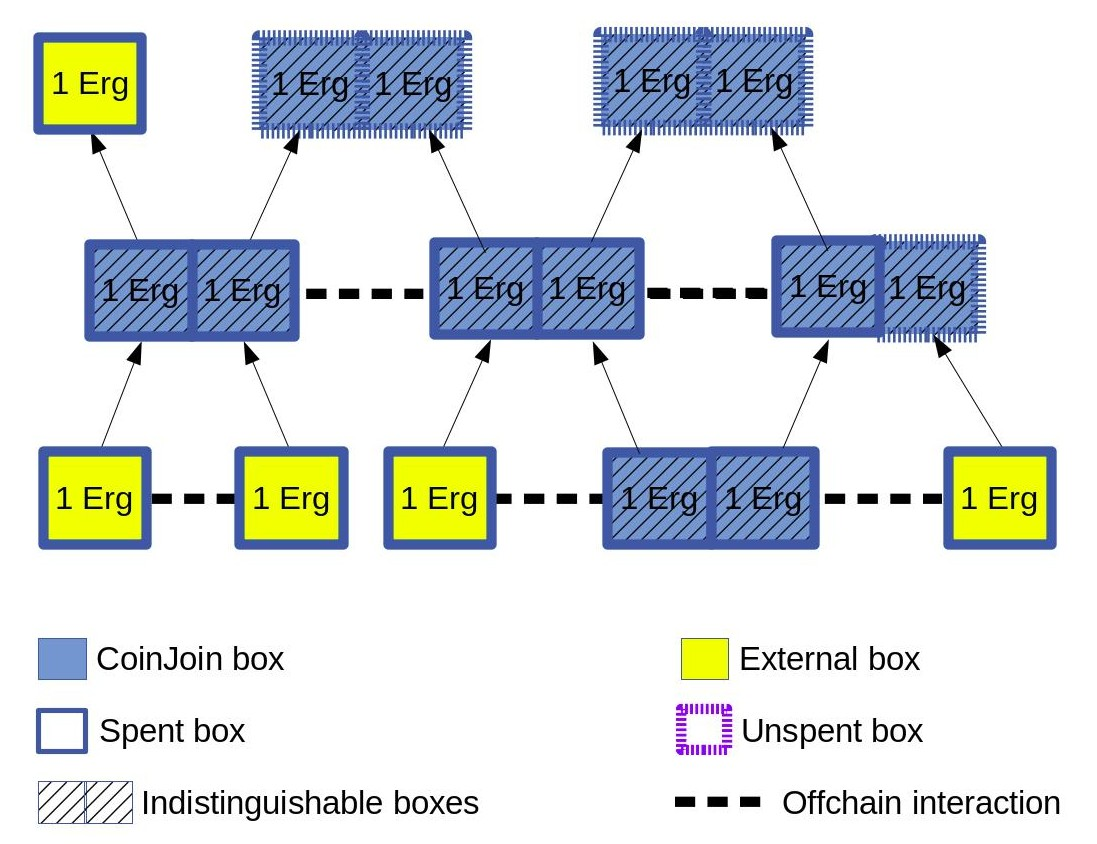
\includegraphics[width=\linewidth]{CoinJoin}
		\captionof{figure}{CoinJoin}
		\label{fig:coinjoin}
	\end{subfigure}%
	\begin{subfigure}{.5\textwidth}
		\centering
		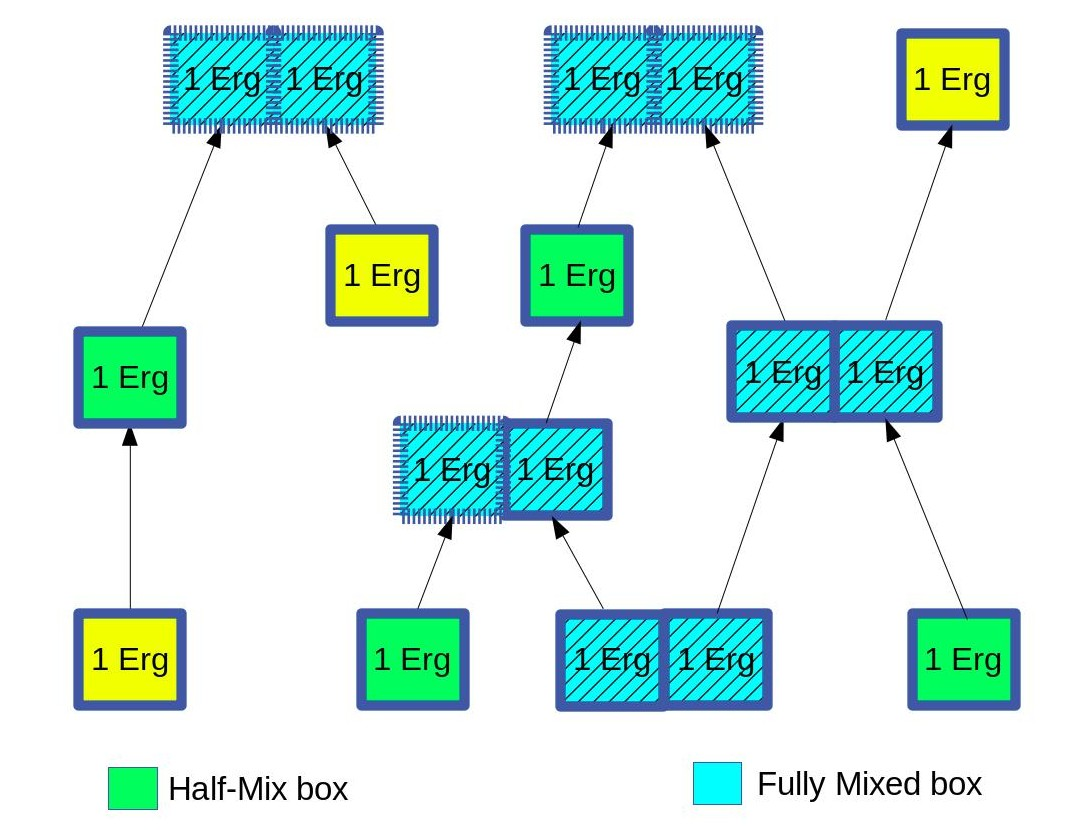
\includegraphics[width=\linewidth]{ErgoMix}
		\captionof{figure}{\mixname}
		\label{fig:mixname}
	\end{subfigure}
	\caption{Comparing CoinJoin and \mixname}
	\label{fig:comparecoinjoin}
\end{figure}

\paragraph{Comparing with ZeroCoin:} ZeroCoin is a privacy enhancing protocol that uses a mixing pool. An ordinary coin is added to the pool as a commitment $c$ to some secrets $(r, s)$, and is later spent such that the link to $c$ is not publicly visible. The value $c$ must be permanently stored in the pool, since the spending transaction cannot reveal it. Instead, it reveals the secret $s$ (the {\em serial number}) along with a zero-knowledge proof that $s$ was used in a commitment from the pool. The serial number is permanently stored to prevent double spending. One consequence of this is that both the pool (the set of commitments) and the set of spent serial numbers must be maintained in memory for verifying every transaction. Another consequence is that the sizes of the these two sets increase monotonously.
This is the main drawback of ZeroCoin (also ZCash~\cite{zcash}), which \mixname tries to address. 
In \mixname, once a box is spent, no information about it is kept in memory, and in particular no data sets of monotonously increasing sizes are maintained. 
%The data storage overhead in \mixname is proportional to the number of unspent boxes, while that of ZC is proportional to the number of deposits (i.e., both spent and unspent boxes).  


\paragraph{Offchain Pool:} The H-Pool can be kept entirely offchain, so that Alice's Half-Mix box need not be present on the blockchain till the time Bob decides to spend it. Alice sends her unbroadcasted transaction directly to Bob who will broadcast both transactions at some later time. 

\paragraph{Future enhancements:} Compared to CoinJoin, \mixname requires an additional box (the Half-Mix box) as depicted in Figure~\ref{fig:comparecoinjoin}. It will be better to have a variant that eliminates this box. 
One way to do this would be to find a way so that the mix step directly outputs two indistinguishable Half-Mix boxes that can be used either in the mix step or spent externally. 
\subsubsection{Handling Fee In \mixname}

%\paragraph{Fixed Value Coins:} 
Similar to ZeroCoin and the canonical variant of CoinJoin in Figure~\ref{fig:coinjoin}, each coin in \mixname must be of a fixed value, which is carried over to the next stage. 
This is fine in theory but implies zero-fee transactions, which is not possible in practice. Below we discuss some approaches for handling fee. 

Assume that fee is paid in {\em mixing tokens}, which are tokens\footnote{Every transaction may generate any quantity of at most one token, whose ID is the box-ID of the first input. For other token-IDs, the sum of quantities in outputs must be less than or equal to the sum of quantities in inputs.} issued by a 3rd party and that creation of a mixed output consumes one such token. A mix transaction (which has two such outputs) consumes exactly two mixing tokens and, to maintain privacy, the balance must be equally distributed between the two outputs. Below are some strategies to ensure fairness in fee payment. 

\begin{enumerate}
	\item \textbf{Perfect Fairness:} 
 Alice's Half-Mix box contains $i$ mixing tokens and she requires each output box to contain $i-1$ mixing tokens. Thus, Alice can mix her coin $i$ times. 
 
 This optimal fee strategy, however, has two drawbacks. Firstly, it has weakened privacy because it restricts the coins that can be mixed. Secondly, it impacts usability because there may not be boxes with the desired number of tokens. The approximate fairness strategy, discussed next, has better privacy and usability at the cost of reduced fairness.
 
 \item \textbf{Approximate Fairness:} Alice relaxes her condition by requiring that Bob contribute at least one token in the mix. %In the worst case, Alice will have to start with $2^i$ tokens to mix $i$ times. 
 However, 
she also requires Bob to have {\em initially} started with exactly 1000 tokens in his first mix. Thus, if Bob is contributing, say, 1 token in the current mix, then Alice wants to ensure that he actually got there `the hard way', by starting out with 1000 tokens and losing them in sequential mixes. %, rather than just by starting out with 1. 
This can be done as follows:

Firstly, the token issuer must restrict the entry of tokens by issuing them only in batches of 1000 in a box protected by the script below,
which requires that the tokens can be transferred (as a whole) only if the transaction is either a mix transaction or creates a Half-Mix box: 
\begin{verbatim}
val halfBox = {(b:Box) => blake2b256(b.propositionBytes) == halfMixScriptHash}
val sameTokenHalfBox = {(b:Box) => halfBox(b) && b.tokens(0) == SELF.tokens(0)}
carol && (halfBox(INPUTS(0) || sameTokenHalfBox(OUTPUTS(0))) // carol is buyer
\end{verbatim}

The value \texttt{halfMixScriptHash} is a hash of \texttt{halfMixScript}, which has the following additional code: 
\texttt{out.R7[Coll[Byte]].get == blake2b256(SELF.propositionBytes)}, thereby ensuring that $R_7$ of each output contains its hash. The code of \texttt{fullMixScript} is modified:

\begin{verbatim}
val halfMixScriptHash = SELF.R7[Coll[Byte]].get
val halfBox = {(b:Box) => blake2b256(b.propositionBytes) == halfMixScriptHash}
val sameTokenHalfBox = {(b:Box) => halfBox(b) && b.tokens(0) == SELF.tokens(0)}
val noToken = {(token:(Coll[Byte], Long)) => token._1 != SELF.tokens(0)._1}
val noTokenBox = {(b:Box) => b.tokens.forall(noToken)}
val noTokenTx = OUTPUTS.forall(noTokenBox)
(halfBox(INPUTS(0)) || sameTokenHalfBox(OUTPUTS(0)) || noTokenTx) && ...
\end{verbatim}
\item \textbf{First Spender Pays Fee:} Another enhancement, primarily in perfect fairness, is to benefit the party that is willing to wait longer. We then require that the fee for the mix transaction be paid by the first party that spends an output. We can identify the first spender as follows. 

A mix transaction must generate exactly 4 quantities of a token (with some id $x$) distributed equally among 4 outputs. Two of these are the standard mix outputs $O_0, O_1$ with the additional spending condition that one output must contain some non-zero quantity of token $x$. The other two boxes, $O_2, O_3$, have the following identical spending conditions:
\begin{enumerate}
	\item The sum of quantities of token $x$ in the inputs and outputs is 3 and 2 respectively.
	\item One output contains 2 quantities of token $x$ protected by the same script as this box. 
\end{enumerate}

Then it the second spender if and only if there is an input with two quantities of token $x$. 
The mix step will create an additional box with two tokens spendable by the second spender.
\end{enumerate}

%Instead of paying fee in tokens, a miner ca accumulate the fee and pay directly in Ergs at the end. This 
 
% \textbf{Fee Accumulation:} Starting with a fixed number of tokens restricts the number of mixes. To allow arbitrary number of mixes, we suggest a {\em fee accumulation} strategy, where the fee is accumulated rather than paid upfront. 
%For instance, fee for the mix transaction can be paid when spending the mixed outputs. 	
% The fee keeps accumulating as long as the coin is circulated within the system (i.e., sent back to the H-pool or used in another mix operation) and is paid when the coin exits the system.

%\section{Finite-State Machine}
\section{Conclusion}

This article described smart contracts written in \langname. The examples build upon concepts from the \langname white-paper~\cite{whitepaper}. More advanced contracts will be discussed in another tutorial.

\bibliographystyle{unsrt}
\bibliography{sigmastate_protocols}
\end{document}